%%==================================================
%% chapter5.tex for BIT Master Thesis
%% version: 0.1
%% last update: Nov 8th, 2017
%%==================================================
\chapter{半参数自适应运动控制}\label{chap:5}
反馈控制是为解决实际问题而研究设计的。前面几章针对一种典型先验信息和数学描述的模型设计了半参数自适应估计与控制器,并用数值仿真验证了控制器性能。本章将考虑半参数自适应控制引入到运动控制场景,解决多关节机械臂中伺服电机的控制问题。
\section{问题描述}\label{chap:5.1}
\subsection{机器人控制}\label{5.1.1}
一般来说,机器人是一个复杂的多输入、多输出非线性系统,具有时变、强耦合和非线性的动力学特征。机器人运动学和动力学的非线性和耦合性使得机器人控制系统的设计十分复杂,一般来说,将如图\ref{fig.robot}所示机器人(机械臂)的运动控制分成两个阶段分别优化,即任务空间的轨迹(路径)规划和关节空间的跟踪控制\upcite{ShinMckay1986}。前者轨迹(路径)规划部分性能的提高涉及到运动学甚至障碍物等约束等多种综合因素的考量,轨迹规划器最终会给后者跟踪控制以关节空间形式提供一段期望的运行轨迹。本章主要考虑关节空间的跟踪控制问题。

\begin{figure}[!htb]
	\centering
	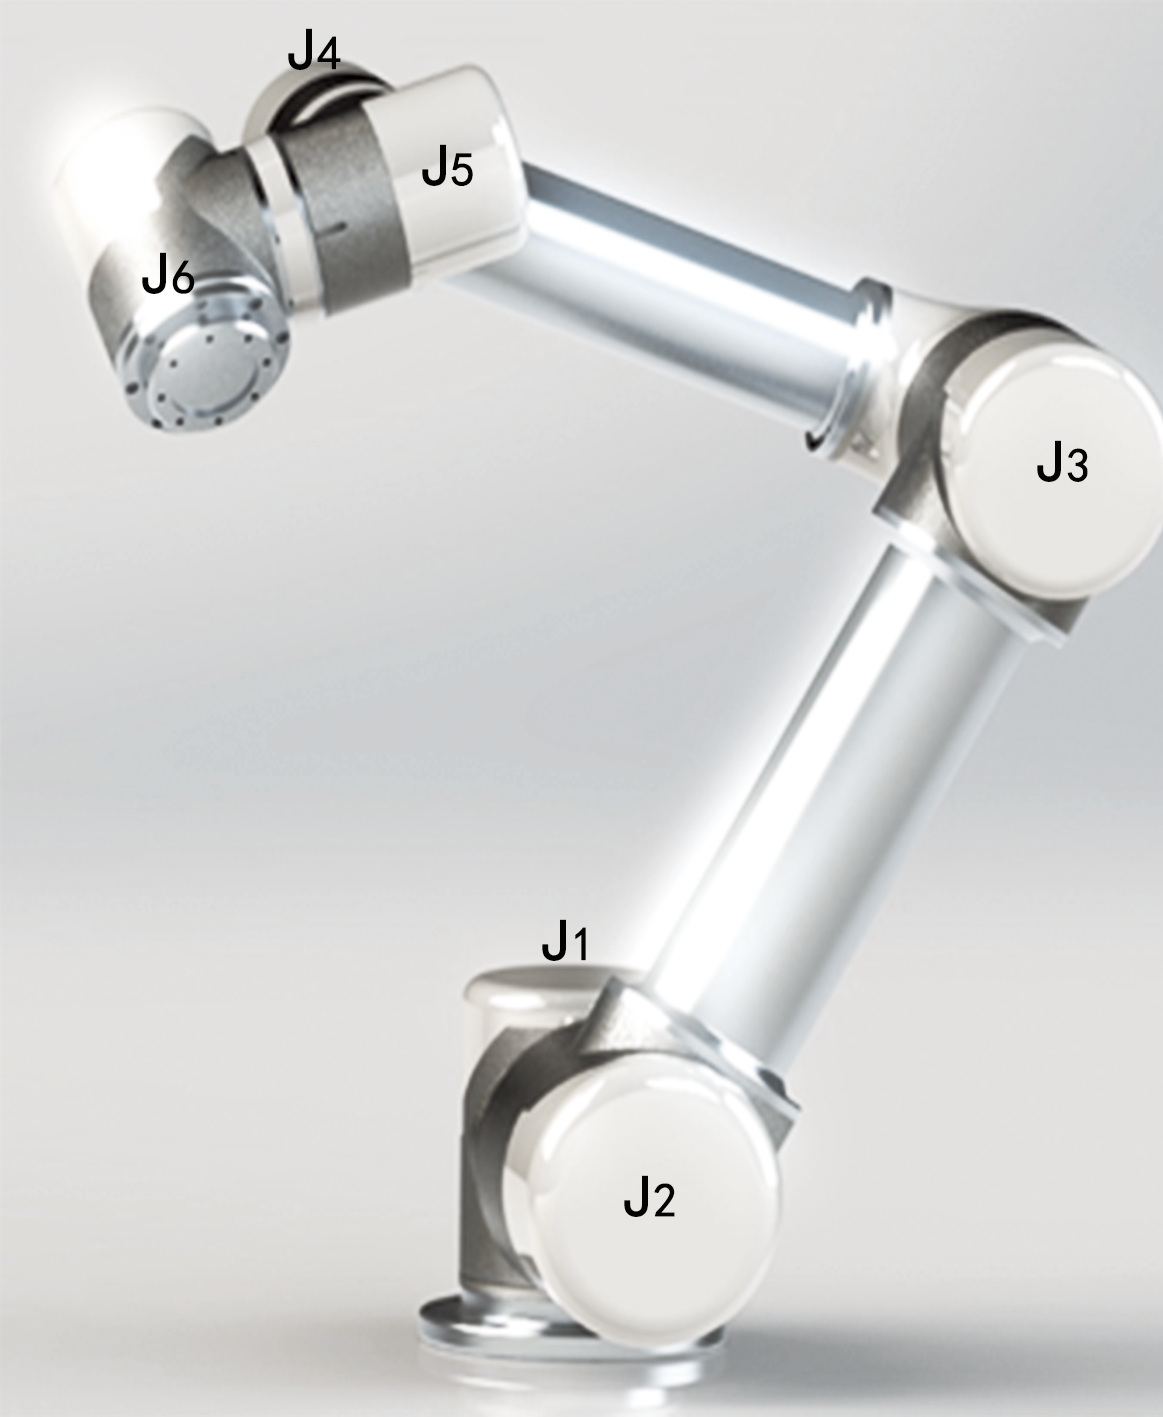
\includegraphics[width=0.35\textwidth ]{ch5-ur-robot.png}\\	 % e.g.,[scale=0.75], [width=0.75\textwidth ]
	\caption{一种UR构型的协作机器人}
	\label{fig.robot}
\end{figure}

工程应用中由于建模和测量的不准确,加上负载的变化以及外部扰动的影响,实际上难以获得机器人精确完整的运动学模型。因此机器人的控制系统中存在的不确定性因素主要可以分为两类,第一类是参数不确定性,如负载质量、连杆长度、连杆质心等物理量未知或部分已知;第二类是非参数不确定性,如高频未建模动态,包括驱动器动力学、结构共振模式,以及低频难以建模动态,如动态/静态摩擦力、关节柔性等。

图\ref{fig.robot}的机器人具有六个自由度,分别由六个关节J1~J的执行机构实现。在无障碍情形下,理论上该机器人的末端可以实现空间任意的位姿,其精度主要表现在任务空间(某个笛卡尔空间)的定位精度。工业高性能的应用场合中,一般要求机器人能达到毫米级的定位精度。机器人的位置控制问题最终要驱动各个关节的电机运动,然后经过减速器等传动机构来实现,因此下面详细讨论单轴的伺服电机控制问题。

\subsection{伺服电机控制}\label{chap:5.1.2}
目前大多数科研、教学和工业应用的机器人都是电力驱动的,一般可分为电压控制和电流控制两种,永磁同步交流伺服电机驱动已成为高性能伺服系统的主要发展方向。对于中小功率机械臂(比如图\ref{fig.robot}所示的协作机器人)的电机建模来说,一般考虑电流控制情形,即电机具有如下的数学模型:
\begin{equation}\label{eq:5.motor}
\begin{array}{c}
i_{c} = K_{a}*u_{c}\\
\tau = K_{m} * i_{c}\\
J_{0}\dot{w} + B \omega + \tau_{f}(\omega) = K_{m} K_{a} u_{c}
\end{array}
\end{equation}
其中,$Q$、$\omega$和$\dot{\omega}$分别是电机输出的角位移(单位是rad)、角速度(单位是rad/s),角加速度($\mathbf{rad/s^{2}}$);$J_{0}$是从电机侧感受到的所有转动惯量之和(包括传动机构和负载等,单位是$\mathbf{kg\cdot m^{2}}$);$B$是粘滞摩擦系数(单位是$\mathbf{N\cdot s}$),$\tau_{f}$是Coulomb摩擦力矩(单位是$N\cdot m$);$K_{a}$和$K_{m}$分别是驱动放大器的导纳系数和电机的力矩常数。

机器人多个关节同时运动时,从单个电机侧感受到的惯量$J_{0}$是时变的。虽然理论上可以通过机器人的动力学模型计算出关节侧的转动惯量值,但是前面一节介绍的不确定性因素的存在,惯量值的计算常常不准确,并且计算十分耗时。不过,经过减速器的传动,从电机侧感受到的关节侧转动惯量时变的效应减小。以一般机器人最大功率的第二个关节$J_{2}$为例(减速比$G$一般为80\~{}150之间),记该轴在机器人动力学模型中惯性矩阵所对应的值为$M_{22}$,则该轴电机侧感受到的所有转动惯量之和为
\begin{equation}\label{eq:5.J0}
J_{0} = J_{m} + \frac{1}{G^{2}}M_{22}
\end{equation}
可以看出,$M_{22}$的变化效应被缩小了$10^{4}$的数量级。然而即使这样,J_{0}的准取值依然难以获得。

上述伺服电机的控制输入可以认为是给定电压(本质是控制输入电流),被控的输出量是角位移或者速度。除了转动惯量的不确定性外,后面的摩擦力项也和角速度等具有是非线性的关系,难以精确建模。如果忽略Coulomb摩擦力矩项,借助于拉普拉斯变换,可以得到电机模型\eqref{eq:5.motor}的传递函数表述式为:
\begin{equation}\label{eq:5.trans}
\frac{\Omega(s)}{U_{c}(s)}=\frac{K_{m}K_{a}}{J_{0}s+B}
\end{equation}
其中$\Omega(s)$和$U_{c}(s)$分别是时域函数$\omega(t)$和$u_{c}(t)$的拉普拉斯变换结果。

方程\eqref{eq:5.trans}是对于速度控制是一阶模型。不过,由于机器人最终控制的是角位移,因此伺服电机系统可以近似为二阶线性模型,可以采用一些常规的线性控制方法,不过它的参数$J_{0}$时变,$B$常常难以知道精确值。现代伺服系统大都采用数字化离散时间控制。记采样周期为$T_{s}$,从离散时间控制角度,在第$k$个时刻电机的输入量和输出量分别记为
$$u_{k}=u_{c}(k\cdot T_{s}),\ y_{k}=\omega(k\cdot T_{s})$$
则系统\eqref{eq:5.motor}的输入输出关系可以写作
\begin{equation}\label{eq:5.nonlinear}
y_{k+1}=F(\bm{\Psi}{k},\epsilon_{k+1})
\end{equation}
其中$\bm{\Psi}_{k}$是输出$y_{k}$和输入$u_{k}$的历史数据组成的回归向量,$\epsilon_{k+1}$是随机干扰。

方程\eqref{eq:5.nonlinear}综合考虑了Coulomb摩擦等所有未建模动态,这样\eqref{eq:5.motor}转化成离散时间后不确定性大大增加,也就是说电机的离散时间模型本质是非常复杂且难以建立准确建模的,也就给直接控制系统带来了很大困难。实际上,伺服电机系统可以采用常规的线性系统方法如PID控制,可以获得一定的控制效果,但是精度和控制特性都有待提高。这从一个侧面反映了\eqref{eq:5.nonlinear}的主体是线性的,只是线性部分参数可能未知,并且含有难以建模的非参数部分。另外,伺服电机含有大量可利用的先验信息,如电机转矩的有界性、惯量变化的有界性等。这十分符合本课题前面提出的半参数系统特性。

\section{控制器设计}\label{chap:5.2}
基于前面小节的分析,本节将应用半参数模型的理论和方法分析机器人中电机运动控制问题,并设计相应的自适应控制器。
\subsection{半参数建模}\label{5.2.1}
结合方程组\eqref{eq:5.motor},电机的角速度$y_{k+1}$主要取决于上一个时刻的角速度$y_{k}$和加速度$a_{k}$。如果记$\tau_{k}$、$\tau_{k,f}$分别为电流产生的力矩和电机运动的摩擦阻力(即$B \omega + \tau_{f}(\omega)$),则电机在$k$时刻的加速度近似为
$$a_{k}=\frac{(\tau_{k}-\tau_{k,f})}{J_{0}}$$
由速度和加速度的微分关系,可以得到电机的角速度$y_{k+1}$为
\begin{equation}\label{eq:5.yk1}
\begin{split}
y_{k+1}&=y_{k}+a_{k}\cdot T_{s}+f'(\bm{\psi}_{k})+\epsilon_{k+1}\\
&=\theta_{1}\cdot y_{k}+\theta_{2}\cdot u_{k}+f(\bm{\psi}_{k})+\epsilon_{k+1}
\end{split}
\end{equation}
其中,$\theta_{1}$未知,可以认为近似为1,而$\theta_{2}$与电机本身参数有关,可以近似为
$$\theta_{2}=\frac{K_{m}K_{a}}{J_{0}}$$
$f(\cdot)$是未知非线性函数,主要融合了难以建模的摩擦和惯量等信息,而$\epsilon_{k+1}$是系的随机干扰。

在系统\eqref{eq:5.yk1}中,$\bm{\theta}=[\theta_{1},\ \theta_{2}]$是系统的参数不确定性部分,维数
$$d_{1}=p_{1}+q_{1}=1+1=2$$
$$\bm{\phi}_{k}=[y_{k},u_{k}]$$
参数部分的先验信息表现为有界性。$\theta_{1}$近似为,可认为取值在0.8到1.2之间;$\theta_{1}$的上下界可以通过分析电机本身的参数$K_{a}$、$K_{m}$的合适范围,以及在机器人运动过程中惯量$J_{0}$的变化范围等数值确定大致范围。

$f(\bm{\psi}_{k})$是系统的非参数不确定性部分,回归向量$\bm{\psi}_{k}=$是历史输入输出数据的组合,即
$$\bm{\psi}_{k}=[y_{k},\ldots,y_{k-p_{2}},u_{k-1},\dots,u_{k-q_{2}+1}]$$
维数$d_{2}=p_{2}+q_{2}$不定,对应的是网络的输入层神经元个数,一般为1到10之间。一般来说,维数$d_{2}$越大,网络训练的数据越多,则逼近效果越好的;但同样过大的维数会加重网络训练的计算量,还会造成过拟合,实际中可以调整选择合适的维数。

系统的非参数不确定性部分的先验信息也表现为有界性。由于离散时间化导致这里的$f(\cdot)$难以直接找到它的变化范围,与前面第三章和第四章的上下界函数有所不同。不过,由于电机本身功率和加速度的限制,电机的速度与前一个时刻相差不会很大,往往在一定范围内,可以认为$f(\bm{\psi}_{k})$满足Lipschitz条件。具体表现为,存在正常数$L_{f}$,使得
\begin{equation}\label{eq:5.flim}
|f(\bm{\psi}_{k-1})-f(\bm{\psi}_{k-})|\leq L_{f}\|bm{\psi}_{k-1}-\bm{\psi}_{k-2}|\|
\end{equation}
对于$k\geq2$都成立。这里,$\|\|$记为向量的某种范数。一般来说,随机干扰序列$\epsilon_{k}$具有有界性,可以认为独立同分布,且取自随机均匀分布。

\subsection{自适应估计}\label{5.2.2}
为了实现半参数自适应控制,首先得设计自适应估计算法。由于半参数系统\eqref{eq:5.yk1}的参数部分也是二维情形,非参数部分也是有界的,可以利用其先验信息借助设计信息浓缩算法估计未知参数。只是有所不同的是,非参数部分的有界形式有所不同,导致算法\ref{alg.ic.2d}和方程\eqref{eq:2.v}中$v_{k,1}$和$v_{k,2}$的计算有所不同。下面给出具体推导过程。

当$k\geq2$,对于任意$0\leq s\leq k-2$,由约束关系\eqref{eq:5.flim}可以得到
\begin{equation}\label{eq:5.flim.s}
|f(\bm{\psi}_{k-1})-f(\bm{\psi}_{s})|\leq L_{f}\cdot\|bm{\psi}_{k-1}-\bm{\psi}_{s}|\|
\end{equation}
而
\begin{equation*}
\begin{split}%
|f(\bm{\psi}_{k-1})-f(\bm{\psi}_{s})|&=(y_{k}-\bm{\theta}^{\tau}\bm{\phi}_{k-1})-(y_{s+1}-\bm{\theta}^{\tau}\bm{\phi}_{s})\\
&=(y_{k}-y_{s+1})-\bm{\theta}(\bm{\phi}_{k-1}-\bm{\phi}_{s})
\end{split}
\end{equation*}
记
$$\Delta_{s}=L_{f}\cdot\|\bm{\psi}_{k-1}-\bm{\psi}_{s}\|$$
再结合\eqref{eq:5.flim.s}得到
\begin{equation}\label{eq:5.}
|\bm{\theta}(\bm{\phi}_{k-1}-\bm{\phi}_{s})-(y_{k}-y_{s+1})| \leq \Delta_{s}
\end{equation}
因此进一步得到线性约束不等式
\begin{equation}\label{eq:5.theta.lim}
(y_{k}-y_{s+1})-\Delta_{s}\leq \bm{\theta}(\bm{\phi}_{k-1}-\bm{\phi}_{s}) \leq \Delta_{s}+(y_{k}-y_{s+1})
\end{equation}

在几何上,式子\eqref{eq:5.theta.lim}就代表了两条直线约束关系,作为每个周期的参数信息集$I_{k}$,可以用来设计信息浓缩估计算法。

\section{仿真实例}

\section{本章总结}
本章主要介绍了